% ---------------------------------------------------------------------------- %
% -------------------------- nevermind the preamble -------------------------- %
% ---------------------------------------------------------------------------- %
\documentclass[10pt,a4paper]{article}
\usepackage[a4paper, total={160mm, 240mm}]{geometry} % smaller margin %
\usepackage[utf8]{inputenc} % umlauts %
\usepackage[german]{babel} % validation %
\usepackage[autostyle]{csquotes}
\MakeOuterQuote{"}


\usepackage{hyperref}

\usepackage{enumitem}
\setlist[enumerate, 1]{label=(\alph*)}
\setlist[enumerate, 2]{label=\arabic*}

\usepackage{titlesec}
\titleformat{\section}[hang]{\small}{\textbf{Task \thesection:}}{.5em}{}

\usepackage{amsmath}
\usepackage{amssymb}

\usepackage{graphicx}
\usepackage[export]{adjustbox}

% ---------------------------------------------------------------------------- %
% -------------------------- nevermind the preamble -------------------------- %
% ---------------------------------------------------------------------------- %

\title{ \vspace{-3em}
        Assignment 03\\
		\small{\bf Digital Libraries and Foundations of Information Retrieval}\\
		\small{Winter semester 2022}}
\author{\small{1542011 Franka Brunen}, \small{1365848 Andreas Schneider}}
\date{}
\begin{document}
\setlength{\parskip}{6pt} % Remove paragraph first line h-indent and instead add v-margin %
\setlength{\parindent}{0pt}

\leftskip=1cm\rightskip=0.5cm % Indent paragraphs for readability %
\setlist[1]{leftmargin=2cm} % Indent first level of lists accordingly %

\maketitle

\section{\hfill Information Needs\hfill 3+6+6 Points}
\begin{enumerate}
    \item \begin{enumerate}
            \item Information on the person "Queen Elizabeth"
            \item Information on the term "queen", as in "queen regnant"
            \item Information on the term "queen", as in the music band
            \item Information on the term "queen", as in the magazine
            \item A disambiguation including all of the above and more like \url{https://en.wikipedia.org/wiki/Queen}
        \end{enumerate}
    \item First 10 results for duckduckgo.com:\\
        \hspace*{-2cm}\begin{tabular}{|p{.73\textwidth}||c|c|c|c|c|c|}
            \hline
            \textbf{Name} & \textbf{1} & \textbf{2} & \textbf{3} & \textbf{4} & \textbf{5} & \textbf{other}\\
            \hline
            Queen (Band) - Wikipedia&&&X&&&\\
            QueenOnline.com - The Official Queen Website&&&X&&&\\
            Queen - Greatest Live Performances - YouTube&&&X&&&\\
            Queen - Bohemian Rhapsody (Official Video Remastered) - YouTube&&&X&&&\\
            Queen | Biografie - Universal Music&&&X&&&\\
            Elisabeth II. - Wikipedia&X&&&&&\\
            Queen Elizabeth (†): Enthüllt! Ihre strikte Regenschirm-Regel&X&&&&&\\
            Beisetzung von Queen Elizabeth II.: ++ Sarg im Familienkreis beigesetzt ...&X&&&&&\\
            Queen-Beerdigung: Der Tag in Bildern - ZDFheute&X&&&&&\\
            Queen - Wikipedia, la enciclopedia libre&&&X&&&\\
            \hline
        \end{tabular}
        
        First 10 results for duckduckgo.com:\\
        \hspace*{-2cm}\begin{tabular}{|p{.73\textwidth}||c|c|c|c|c|c|}
            \hline
            \textbf{Name} & \textbf{1} & \textbf{2} & \textbf{3} & \textbf{4} & \textbf{5} & \textbf{other}\\
            \hline
            Queen (band) - Wikipedia&&&X&&&\\
            Elizabeth II - Wikipedia&X&&&&&\\
            Queen The Band Now Worth More Than The Queen Of England - Audacy&X&&X&&&\\
            Adam Lambert confesses fear of following Freddie Mercury before ...&&&X&&&\\
            Queen + Adam Lambert - Wikipedia&&&X&&&\\
            Behind the Band Name: Queen - American Songwriter&&&X&&&\\
            Queen Official - YouTube&&&X&&&\\
            QueenOnline.com - The Official Queen Website&&&X&&&\\
            Queen | Spotify&&&X&&&\\
            Queen - Facebook&&&X&&&\\
            \hline
        \end{tabular}
        
        Aggregation of results:\\
        \begin{tabular}{|l||c|c|c|c|c|c|}
            \hline
            & \textbf{1} & \textbf{2} & \textbf{3} & \textbf{4} & \textbf{5} & \textbf{other}\\
            \hline
            \textbf{duckduckgo.com} & 4&0&6&0&0&0\\
            \textbf{google.com} & 2&0&9&0&0&0\\
            \hline
        \end{tabular}
        
        In one case, row 3 from google.com, an article could be assigned to two information needs: \textbf{a} and \textbf{c}.
    \item \begin{enumerate}
            \item "queen" + " elizabeth"\\
                $\rightarrow$ \texttt{10  0  0  0  0  0}
            \item "queen" + " regnant"\\
                $\rightarrow$ \texttt{ 1  5  0  0  0  4}
                \\(with two "other" being info on queens other than Elizabeth II and two being lists of queen regnants)
            \item "queen" + " band"\\
                $\rightarrow$ \texttt{ 0  0 10  0  0  4}
            \item "queen" + " magazine"\\
                $\rightarrow$ \texttt{ 2  0  3  4  0  1}\\
                (with "other" being "GUIDOS DEKO QUEEN - das Magazin für alle Deko-Fans"; the Term "magazine" is obviously not very effective in discerning the old UK Queen Magazine)
            \item "queen" + " disambiguation"\\
                $\rightarrow$ \texttt{ 0  0  1  0  3  6}\\
                (with all "other" being disambiguation wiki pages of fictional universes)
        \end{enumerate}
\end{enumerate}


\section{\hfill Precision and Recall\hfill 5+5+5 Points}
\begin{enumerate}
    \item \textbf{Information need:} The difference between \texttt{\textbackslash tabular} and \texttt{\textbackslash tabular*}\\
        \textbf{Search query:} "\texttt{tabular} vs \texttt{tabular*}"
        \begin{figure}[h]
            \centering
            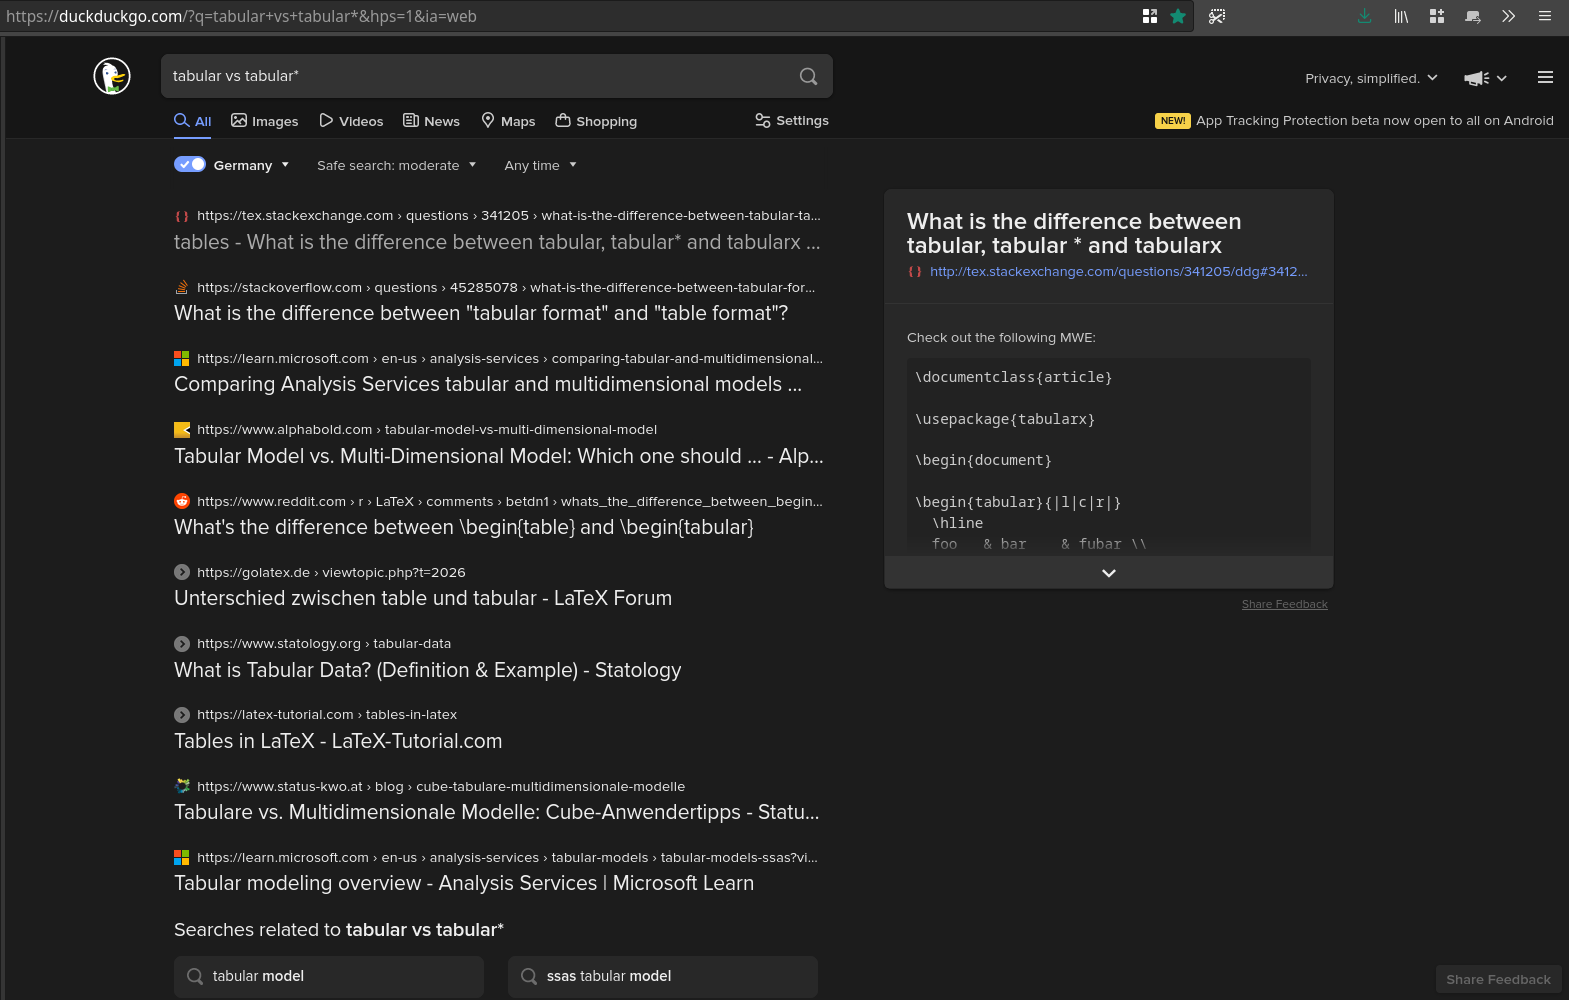
\includegraphics[width=\linewidth]{e03screenshot}
        \end{figure}
    \item \textbf{Precision:} $1/10=0.1=10\% $
    \item One could say that the data to be searched is infinite, as new web pages are indexed at every moment. Therefore the amount of false negatives is unknown.
    
    Between two or more search engines, one can accumulate all the true positives and compare the amount of false negatives of each search engine. If one true positive is returned by one search engine but not the other, the other has a false negative.
\end{enumerate}


\newpage
\section{\hfill Additional evaluation metrics\hfill 4+6+5 Points}
\begin{enumerate}
    \item Definitions:\\
        - $F_\beta$ "is a measure of a test's accuracy. It is calculated from the precision and recall of the test" \footnote{Wikipedia \url{https://en.wikipedia.org/wiki/F-score}}\\
        - \textit{Fallout} is "the fraction of non-relevant documents that are retrieved $ \frac{|ret\cap \neg rel|}{|\neg rel|} $" \footnote{L. Egghe (2008) The measures precision, recall, fallout and miss as a function of the number of retrieved documents and their mutual interrelations \url{https://www.sciencedirect.com/science/article/pii/S0306457307001598}}
        
        The impact of the parameter $\beta$ is that it defines the weight of recall in relation to precision. In other words, recall is weighed "$\beta$ times as much" as precision.
        
        Explanations
        \begin{itemize}
            \item $F_\beta=0$ is possible and means that no relevant document was retrieved.
            \item $F_\beta=1$ is possible and means that no non-relevant document was retrieved and either $\beta$ or the number of non-retrieved relevant documents is $0$.
            \item $Fallout=0$ is possible and means no non-relevant documents were retrieved.
            \item $Fallout=1$ is possible and means all non-relevant documents were retrieved.
        \end{itemize}
    \item Determinations:
    
        \begin{tabular}{l|l|l|l|l}
            Result set&\textit{Recall}&\textit{Precision}&\textit{Fallout}&$F_1$\\
            \hline
            $S_1$ &4/9   &0.40 = 4/10   &5/21   &0.53 = 10/19\\
            $S_2$ &7/9   &0.54 = 7/13   &6/21   &0.64 = 14/22\\
            $S_3$ &6/9   &0.75 = 6/8   &2/21   &0.71 = 12/17\\
        \end{tabular}
        
        In terms of these metrics, $S_3$ is the best-performing one. With this specific search query and document collection, the IR retrieved most relevant results and few non-relevant ones. Only in $Recall$ is $S_2$ better, but not enough to compensate for the false positive and -negatives that affect its $F_\beta$.
    \item Assuming that there is always 1 relevant and 1 non-relevant document to any search query:
        \begin{itemize}
            \item An IR system that retrieves all documents on every query would always have a recall of 1, as it would always retrieve all relevant documents.
            
            Its precision would always be $\frac{rel}{|D|}$; relevant documents divided by the amount of all documents, as it would always return all relevant documents alongside all others.
            
            Its fallout would always be 1, as all documents contain all non-relevant documents.
            \item An IR system that retrieves no documents on every query would always have a fallout of 0, as it would never retrieve any non-relevant document.
            
            Its recall would always be 0, as it would always return 0 relevant documents.
            
            Its precision would always be 0, as it would always return 0 relevant documents.
        \end{itemize}
\end{enumerate}


\end{document}